\documentclass[class=article, crop=false]{standalone}
\usepackage{my_preamble}
\begin{document}
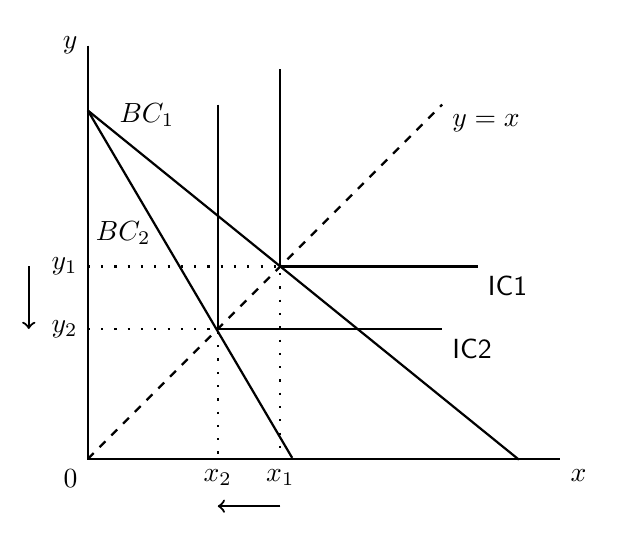
\begin{tikzpicture}[thick,font=\sffamily,scale=1.5]
	%axis
	\draw (0,3.5) node[left]{$y$} -- (0,0) node[below left] {$0$} -- (4,0) node[below right]{$x$};
	
	%graphs	
	\draw plot[domain=0:3.65,smooth] (\x,2.95-0.81*\x); %BC1
	\draw plot[domain=0:1.73,smooth] (\x,2.95-1.7*\x); %BC2
	\draw (1.63,3.3) node[left]{} -- (1.63,1.63) node[below left] {} -- (3.3,1.63) node[below right]{IC1}; %IC1
	\draw (1.1,3) node[left]{} -- (1.1,1.1) node[below left] {} 
	  -- (3,1.1) node[below right]{IC2}; %IC2
	\draw[dashed] (0,0) -- (3,3); %y=x dotted line	
	
	
	\draw[loosely dotted] (0,1.63) node[left]{$y_1$} -| node[pos=0.25,below=3mm] {} (1.63,0) node[below]{$x_1$}; %dotted lines 1
	\draw[loosely dotted] (0,1.1) node[left]{$y_2$} -| node[pos=0.25,below=3mm] {} (1.1,0) node[below]{$x_2$}; %dotted lines 2
	
	%labels and arrows
	\node[below] at (0.5,3.1) {$BC_{1}$}; %BC1 label
	\node[below] at (0.3,2.1) {$BC_{2}$}; %BC2 label
	%\node[below] at (2.8,1.3) {$IC_{1}$}; %IC1 label
	%\node[below] at (2.4,0.6) {$IC_{2}$}; %IC2 label
	\node[below right] at (3,3) {$y=x$}; %y=x label
	
	\draw [->] (1.63,-0.4) -- (1.1,-0.4); %x arrow
	\draw [->] (-0.5,1.63) -- (-0.5,1.1); %y arrow
\end{tikzpicture}
\end{document}